%---------------------------------------------------------------------------------------------------
% Einführung
%---------------------------------------------------------------------------------------------------
\newpage

\section{Einführung}

Die Raumfahrt ist der Versuch der Beherrschung komplexer Technologie.
Dennoch geschehen Unfälle, die gerade in der Start- und Landephase für Gerät und Astronauten katastrophal enden.
Die letzten Unglücke mit umgekommenen Personen waren die Space Shuttles Columbia im Jahre 2003 und Challenger im Jahre 1986.
Im Falle der Challenger gibt es Stimmen, die behaupten, dass die Crew mit einem Rettungssystem hätte überleben können.
Ein Rettungszenario wäre Ausstieg, freier Fall bis in dichtere Atmosphärenschichten und Landung mittels Fallschirm.
Gesteigertes Interesse an der Sicherheit gibt es angesichts der zunehmenden privaten Raumfahrt und der Vision Privatpersonen als Touristen in den Orbit zu transportieren.

\begin{figure}[h]
  \centering
  \begin{subfigure}[b]{0.25\textwidth}
    \centering
    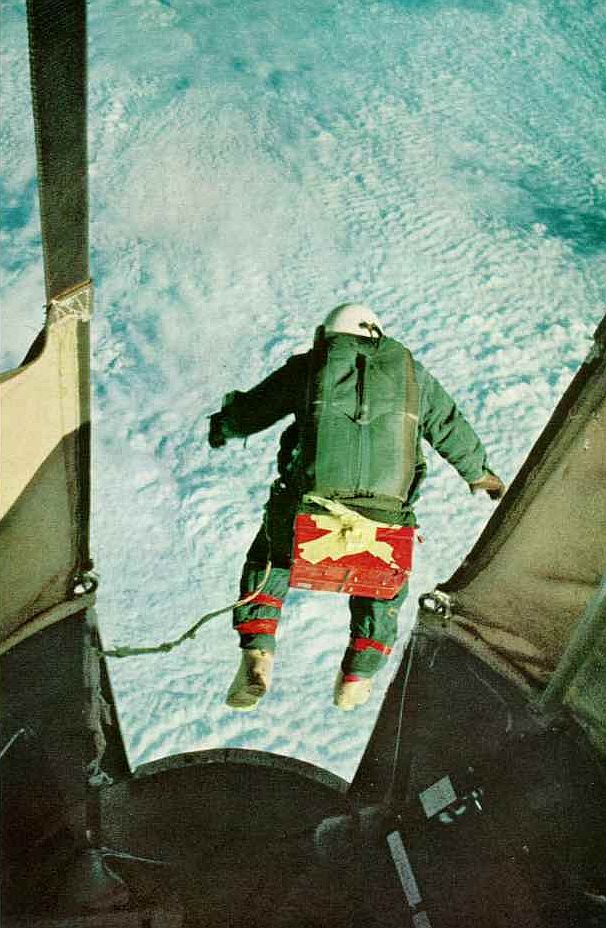
\includegraphics[width=1\textwidth]{excelsior-III-d}
    \caption{Joseph Kittinger\protect\footnotemark}
    \label{fig:excelsior-III-d}
  \end{subfigure}
  ~
  \begin{subfigure}[b]{0.25\textwidth}
    \centering
    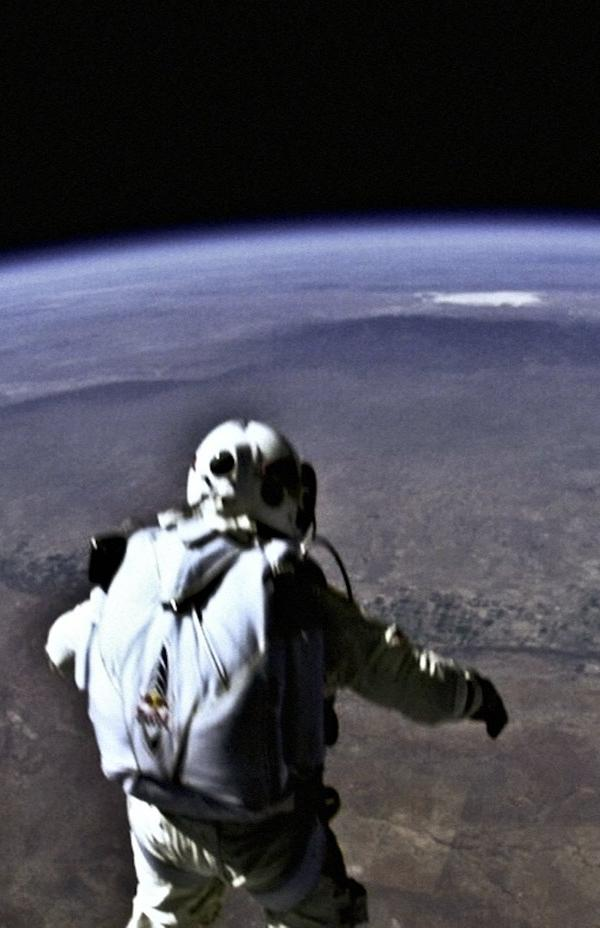
\includegraphics[width=1\textwidth]{baumgartner}
    \caption{Felix Baumgartner\protect\footnotemark}
    \label{fig:baumgartner}
  \end{subfigure}
  \caption{Absprung}
\end{figure}
\footnotetext[1]{Bildquelle: \url{http://stratocat.com.ar/fichas-e/1960/HMN-19600816.htm}}
\footnotetext{Bildquelle: \url{http://www.redbullstratos.com/gallery/}}

Der Fallschirmsprung aus der Stratosphäre wurde unter anderem im Rahmen des Projekts \emph{Excelsior}~\cite{af.mil:excelsior} bereits in den Jahren 1959 und 1960 getestet.
Hierbei lag der Fokus allerdings mehr auf Rettungstrategien für die Besatzungen hoch fliegender Jets.
Grundlegend wurde hierbei bereits die Machbarkeit von Fallschirmsprüngen aus einer Höhe von $30km$ bewiesen.
Der damalige Springer Joseph Kittinger führte drei Sprünge durch.
Es gibt umstrittene Behauptungen, dass er beim letzten Sprung aus $31.333m$ Höhe die Schallmauer durchbrochen hat.
Seit 2009 ist Kittinger am Red Bull Projekt beteiligt und half beratend beim Brechen seiner eigenen Rekorde mit.

Der Getränkehersteller Red Bull hat in den letzten Jahren ein Projekt finanziert, dass in den medienwirksamen Sprung des Österreichers Felix Baumgartners am 14.10.2012 mündete~\cite{rbstratos}.
Er stieg in einer Kapsel mittels Heliumballon in eine Höhe von $39.045m$ auf (geplant waren mindestens $35.576m$) und sprang.
Der Sprung stellte neue Rekorde auf, zum Beispiel das diesmal eindeutig belegte Durchbrechen der Schallmauer ohne Flugzeug im freien Fall.
Weiterhin wurde erneut der Beweis erbracht, dass der Sprung aus derartigen Höhen möglich und dieser Weg als Rettungstrategie denkbar ist und medizinische Daten gesammelt.

Um die Frage zu klären, welche Absprunghöhe nötig ist, um die Schallmauer zu durchbrechen, soll das Experiment simuliert werden.
Dabei soll untersucht werden, wie der Sprung aus unterschiedlichen Höhen verlaufen wäre und welche Faktoren dabei eine Rolle spielen.
Weiterhin wird gezeigt, welche Geschwindigkeit bei einem ungebremsten Fall auf Höhe der Erdoberfläche erreicht wird.

In Kapitel \ref{sec:modellierung} wird auf die Modellierung des Sprungs eingegangen, wirkende Kräfte und gewählte Parameter beschrieben. Das Kapitel \ref{sec:simulation} beschreibt den Aufbau der Simulation, Kapitel \ref{sec:auswertung} wertet die Ergebnisse aus.
% Das Überschreiten vermeintlicher Grenzen gepaart mit Neugier (und die Aussicht auf Ruhm) sind ein starker Antrieb des Menschen.
% Luft- und Raumfahrt sind eine Frucht dieser Motive.
% Trotz aller Vorkehrungen werden hierbei Risiken eingegangen.
% Im Falle der Raumfahrt zwar nur von einigen wenigen Menschen, trotzdem gibt es Bestrebungen hier die Sicherheit zu erhöhen.
% Red Bull hat hierzu medienwirksam ein Experiment finanziert:
% Der Sprung des österreichischen Felix Baumgartners aus einer geplanten Höhe von 36.576m.
% Neben der Werbewirkung und dem Aufstellen neuer Rekorde sollten dabei medizinische Daten gesammelt und die Machbarkeit eines Notausstiegs von Astronauten in großer Höhe und der Rückkehr im freien Fall getestet werden.
